
% this file is called up by thesis.tex
% content in this file will be fed into the main document
%----------------------- introduction file header -----------------------
%%%%%%%%%%%%%%%%%%%%%%%%%%%%%%%%%%%%%%%%%%%%%%%%%%%%%%%%%%%%%%%%%%%%%%%%%
%  Capítulo 1: Introducción- DEFINIR OBJETIVOS DE LA TESIS              %
%%%%%%%%%%%%%%%%%%%%%%%%%%%%%%%%%%%%%%%%%%%%%%%%%%%%%%%%%%%%%%%%%%%%%%%%%

\chapter{\textcolor{Azul}{Introducción}}

%: ----------------------- HELP: latex document organisation
% the commands below help you to subdivide and organise your thesis
%    \chapter{}       = level 1, top level
%    \section{}       = level 2
%    \subsection{}    = level 3
%    \subsubsection{} = level 4
%%%%%%%%%%%%%%%%%%%%%%%%%%%%%%%%%%%%%%%%%%%%%%%%%%%%%%%%%%%%%%%%%%%%%%%%%
%                           Presentación                                %
%%%%%%%%%%%%%%%%%%%%%%%%%%%%%%%%%%%%%%%%%%%%%%%%%%%%%%%%%%%%%%%%%%%%%%%%%

\section{Presentación} % section headings are printed smaller than chapter names

\textcolor{Azul}La primera concepción de la palabra robot proviene de la obra \textit{Rossum's Universal Robots} del novelista checo Karel Capek[1]. En la lengua checha \textit{robota} significa trabajo, y la RAE [2] define a un robot como \textit{Máquina o ingenio electrónico programable, capaz de manipular objetos y realizar operaciones antes reservadas solo a las personas}. \\\\En la industria, los robots  más utilizados son conocidos como robots manipuladores, cuya estructura se asemeja a los brazos humanos, Fig. (\ref{estructurarobot}) [3]. Se estructura está formada por eslabones unidos mediante articulaciones para brindar libertad de movimiento en el entorno de trabajo, donde uno de los extremos del manipulador permanece fijo mientras que el otro extremo cuenta con una herramienta que le permite realizar una tarea para la que fue programado. Los robots manipuladores son utilizados en gran parte de las tareas como seleccionar y distribuir objetos, o para realizar modificaciones en su entorno como pintar o ensamblar, entre muchas otras, reduciendo los tiempos de operación y minimizando la necesidad de supervisión.\\\\Un robot manipulador se constituye de cuatrp sistemas fundamentales. El primero es un sistema mecánico que le da forma al cuerpo del robot y está constituido pricipalmente por eslabones y articulaciones que permiten el movimiento en su espacio de trabajo, aunque también forman parte del sistema mecánico elementos de transmisión de potencia, como engranes, cadenas y poleas; elementos que otorgan estabilidad al robot, como los sistemas de contrapesos, ya sean fijos o móviles; y elementos de unión, como soldadura y tornillos. El segundo es un sistema eléctrico-electrónico que otorga energía para el movimiento de los motores, para la activación de sensores y la distribución de señales. El tercer sistema pertenece a la programación, que constituye la comunicación entre el humano y la máquina. El cuarto  sistema es de control, que describe de manera matemática al robot y permite su manipulación para la realización de una tarea asignada.

\begin{figure}
	\centering
	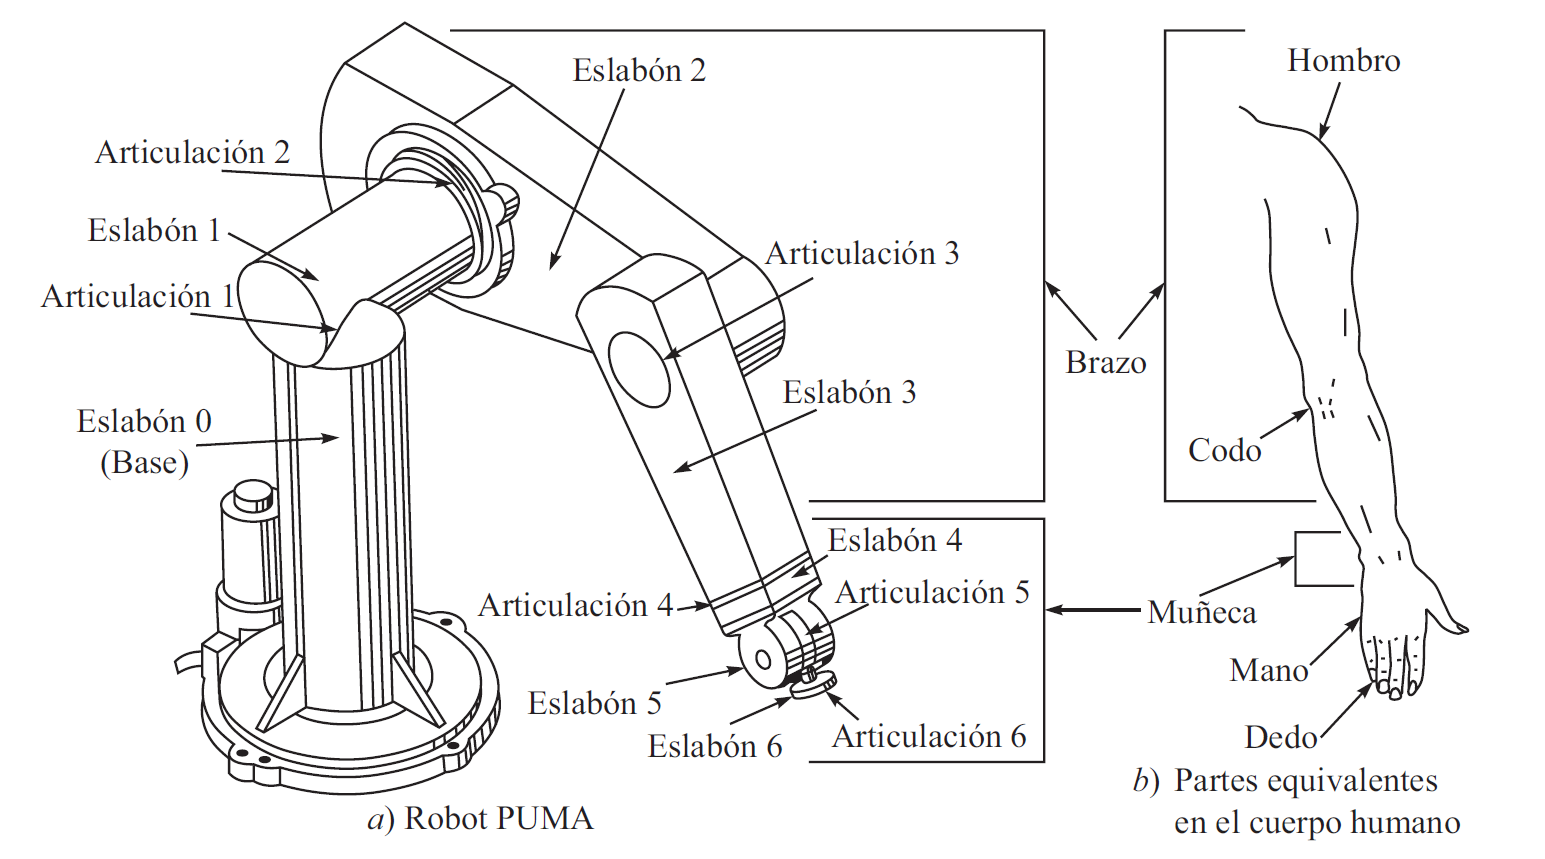
\includegraphics[scale=0.5]{Capitulo1/figs/EstructuraManipulador.png} 
	\caption{Manipulador robótico y sus partes equivalentes en el cuerpo humano}
	\label{estructurarobot}
\end{figure}



%%%%%%%%%%%%%%%%%%%%%%%%%%%%%%%%%%%%%%%%%%%%%%%%%%%%%%%%%%%%%%%%%%%%%%%%%
%                           Objetivo                                    %
%%%%%%%%%%%%%%%%%%%%%%%%%%%%%%%%%%%%%%%%%%%%%%%%%%%%%%%%%%%%%%%%%%%%%%%%%

\subsection{Objetivo}

Diseño y manufactura de un robot manipulador con 5 grados de libertad capaz de realizar seguimiento de trayectorias.
%%%%%%%%%%%%%%%%%%%%%%%%%%%%%%%%%%%%%%%%%%%%%%%%%%%%%%%%%%%%%%%%%%%%%%%%%
%                           Motivación y estado del arte                %
%%%%%%%%%%%%%%%%%%%%%%%%%%%%%%%%%%%%%%%%%%%%%%%%%%%%%%%%%%%%%%%%%%%%%%%%%
\subsection{Motivación}

Los robots manipuladores tienen un amplio uso en la industria y en áreas donde se pretende replicar el trabajo que realiza una persona, ya sea porque es demasiado complejo o se trata de procesos donde se requiera una gran precisión, por encontrarse en ambientes peligrosos o tóxicos, etc. Sin embargo, los robots manipuladores también pueden ser de gran utilidad en el ámbito educativo. Los estudiantes de robótica suelen tener acceso nulo o restringido a manipuladores ya sea por su delicadeza o por la intención de no dañar al robot debido a los elevados costos de reparación. La creación de un manipulador con 5 grados de libertad a un bajo costo pondrá al alcance de los estudiantes una herramienta práctica en el área de la robótica industrial.
%%%%%%%%%%%%%%%%%%%%%%%%%%%%%%%%%%%%%%%%%%%%%%%%%%%%%%%%%%%%%%%%%%%%%%%%%
%                   Planteamiento del problema                          %
%%%%%%%%%%%%%%%%%%%%%%%%%%%%%%%%%%%%%%%%%%%%%%%%%%%%%%%%%%%%%%%%%%%%%%%%%

\subsection{Planteamiento del problema}

El diseño de robots manipuladores es una temática ampliamente abarcada en los trabajos escolares de nivel licenciatura, aunque la mayor parte de esa literatura tiene por objetivo demostrar conceptualmente las capacidades de los robots manipuladores. La construcción del prototipo funcional es un elemento que no se suele llevar a término.
%%%%%%%%%%%%%%%%%%%%%%%%%%%%%%%%%%%%%%%%%%%%%%%%%%%%%%%%%%%%%%%%%%%%%%%%%
%                           Metodología                                 %
%%%%%%%%%%%%%%%%%%%%%%%%%%%%%%%%%%%%%%%%%%%%%%%%%%%%%%%%%%%%%%%%%%%%%%%%%
\subsection{Metodología}

El proceso de construcción del manipulador comienza con el diseño, para ello se plantean los requerimientos y se traducen a especificaciones del robot. Posteriormente se elabora un diseño asistido por computadora donde se obtiene la geometría y espacio de trabajo del manipulador. Se realiza la descripción analítica del movimiento mediante la cinemática directa e inversa, y se termina con la construcción de las piezas y el ensamble del prototipo.

%%%%%%%%%%%%%%%%%%%%%%%%%%%%%%%%%%%%%%%%%%%%%%%%%%%%%%%%%%%%%%%%%%%%%%%%%
%                         Contribuciones                                %
%%%%%%%%%%%%%%%%%%%%%%%%%%%%%%%%%%%%%%%%%%%%%%%%%%%%%%%%%%%%%%%%%%%%%%%%%

\subsection{Contribuciones}

La principal contribución de este trabajo es la simplificación del proceso de construcción para un robot manipulador con 5 grados de libertad, con los elementos necesarios para ser replicado en posteriores trabajos y reduciendo los costos asociados a la fabricación.

%%%%%%%%%%%%%%%%%%%%%%%%%%%%%%%%%%%%%%%%%%%%%%%%%%%%%%%%%%%%%%%%%%%%%%%%%
%                           Estructura de la tesis                      %
%%%%%%%%%%%%%%%%%%%%%%%%%%%%%%%%%%%%%%%%%%%%%%%%%%%%%%%%%%%%%%%%%%%%%%%%%

\subsection{Estructura de la tesis}

En este capítulo se hace una breve descripción del trabajo a desarrollar, el objetivo y algunas ideas generales de robots manipuladores, en el siguiente capítulo se encuentran los fundamentos teóricos que sirven para entender las generalidades de los manipuladores, su composición y la forma de operarlos. En el tercer capítulo se aborda el diseño mecánico junto con un análisis de los elementos que conforman al manipulador, las geometrías y los espacios de trabajo que definirán la movilidad. En el capítulo cuatro se lleva a cabo la construcción del prototipo y la puesta en marcha. En el quinto capítulo se analizan los resultados obtenidos donde se observa la capacidad real del robot manipulador construido y en el último capítulo se tratan las conclusiones y el posible trabajo a futuro del proyecto.

\section{Marco teórico}

Los robots actuales tienen sus orígenes en máquinas controladas remotamente por un operador (teleoperadores) y por máquinas-herramienta controladas numéricamente. A pesar de que el primer teleoperador fue desarrollado en 1947 no fue hasta la década de los 60's cuando los robots manipuladores se incrustaron con éxito en la industria, debido a su alta confiabilidad, repetibilidad y capacidad de adaptación a numerosas actividades. Debajo se encuentra una lista con acontecimientos importantes en el desarrollo de robots manipuladores desde sus inicios al presente.\\\\
1947 - Desarrollo del primer teleoperador servo-eléctrico. El esclavo era servo-controlado para seguir la trayectoria del maestro, sin realimentación.\\\\
1948 - Introducción de un sistema de realimentación en el que la fuerza ejercida por el esclavo era transmitida de vuelta al operador.\\\\
1949 - La Fuerza Aérea de los Estados Unidos patrocinó investigaciones en el desarrollo de herramientas controladas numéricamente. La investigación se realizó para combinar la experiencia en servo-sistemas sofisticados con las recién desarrolladas técnicas de computación digital.\\\\
1954 - George Devol registra una patente en transferencia programada de artículos, Fig (\ref{unimation}).\\\\
1961 - Desarrollo del primer brazo teleoperado equipado con sensores de contacto para dar realimentación de fuerza al operador.\\\\
\begin{figure}[h!]
	\centering
	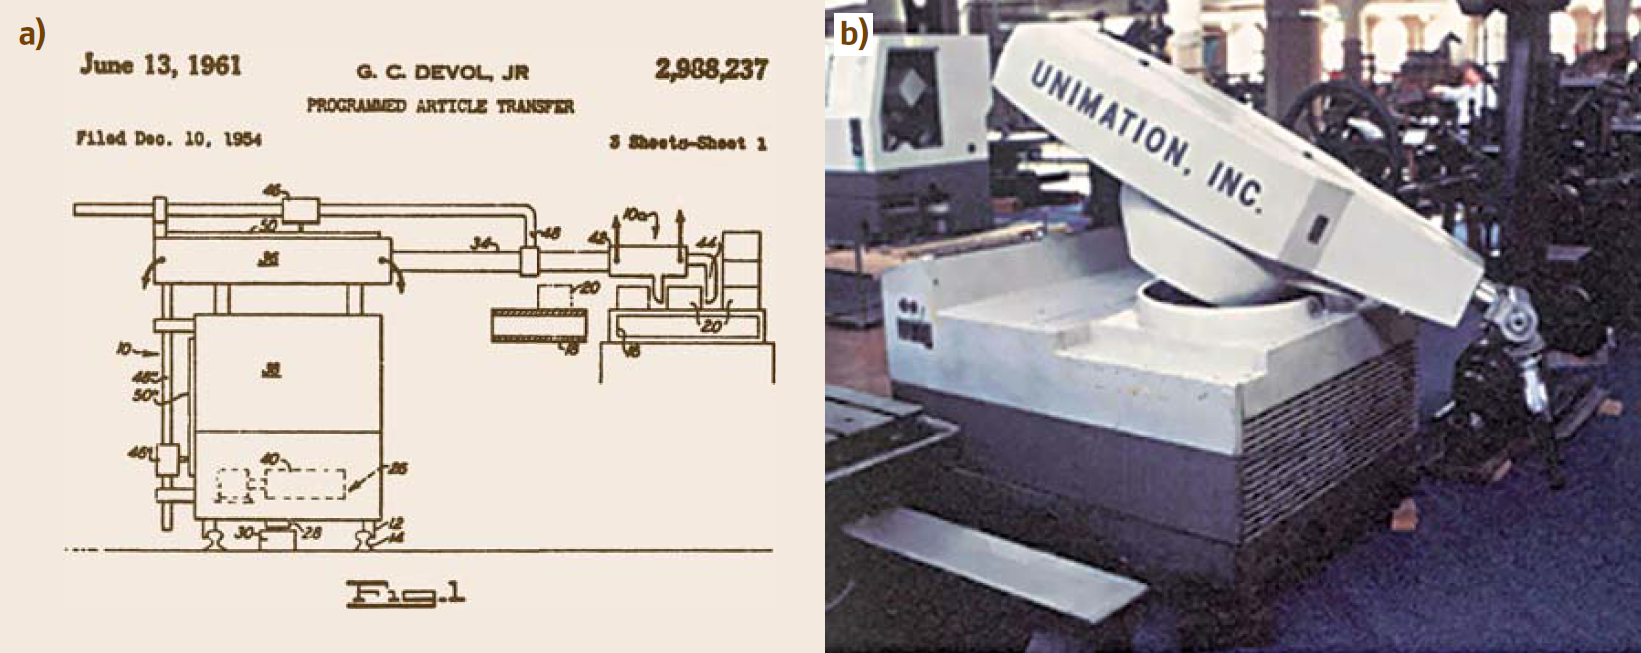
\includegraphics[scale=0.4]{Capitulo1/figs/Unimation.PNG} 
	\caption{(a) La patente de G. Devol marcó el comienzo del trabajo en conjunto con J. Engelberer para crear la primera compañía de robótica del mundo (b) El primer robot instalado en una planta de \textit{General Motors}.}
	\label{unimation}
\end{figure}\\
1963 - Lawrence G. Roberts demuestra la factibilidad de integrar sistemas de visión en los robots.\\\\
1969 - Victor Scheinman diseña \textit{The Stanford Arm}, uno de los primeros manipuladores en ser concebidos exclusivamente para control por computadora. Fig(\ref{stfarm})\\
\begin{figure}[h!]
	\centering
	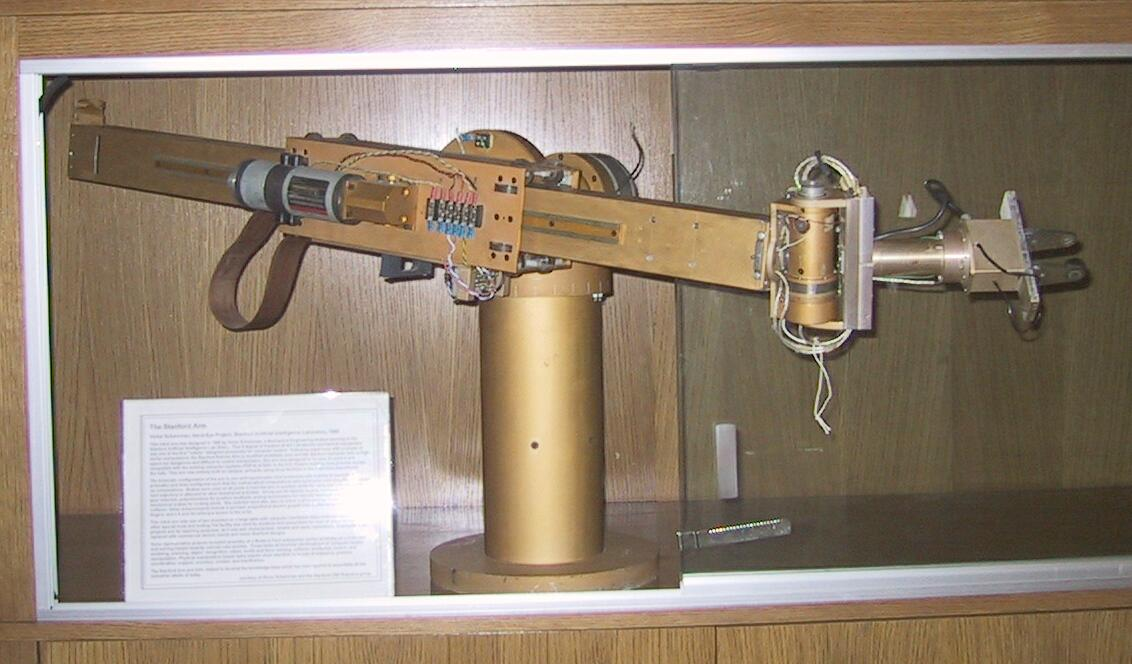
\includegraphics[scale=0.3]{Capitulo1/figs/StanfordArm.jpg} 
	\caption{\textit{The Stanford Arm}. La configuración no es antropomórfica, cuenta con 6 pares cinemáticos (5 rotacionales, 1 prismático).}
	\label{stfarm}
\end{figure}\\
1973 - Creación del primer lenguaje de programación para robots \textit{WAVE} en la Universidad de Stanford.\\\\
1974 - La compañía Cincinnati Milacron introduce el robot T3 con control por computadora integrado. Fig(\ref{puma}) (a).\\\\
1978 - Unimation introduce el robot PUMA, cuya destreza se asemeja a la de un brazo humano. Fig(\ref{puma}) (b).\\
\begin{figure}
	\centering
	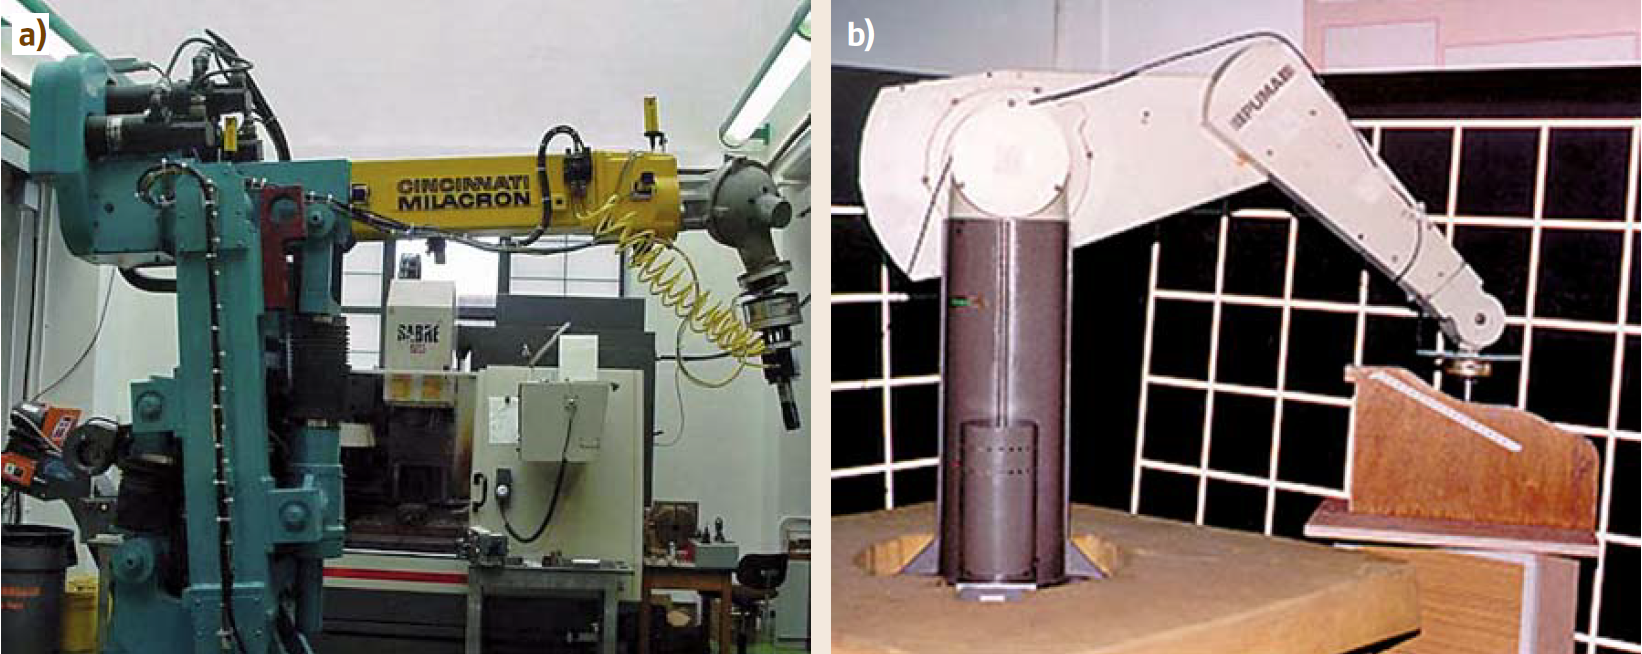
\includegraphics[scale=0.4]{Capitulo1/figs/puma.PNG} 
	\caption{(a) El robot T3 inició con actuadores hidráulicos, para luego ser reemplazados por motores eléctricos (b) El robot PUMA se convierte en una referencia para la investigación en robótica}
	\label{puma}
\end{figure}\\
1978 - El diseño de bajo costo del robot SCARA de 4 ejes marca innovación en la industria al permitir ensamblajes de partes pequeñas a gran velocidad.\\\\
1981 - La Universidad Carnegie Mellon desarrolla el primer robot que utiliza manejo directo.\\\\
1986 - Exploración de los restos de la embarcación\textit{Titanic} con el robot submarino Jason.\\\\
1988 - Creación de la \textit{IEEE RAS} (Sociedad de Robótica y Automatización del Instituto de Ingenieros Eléctricos y Electrónicos, por sus siglas en inglés).\\\\
1993 - El robot experimental ROTEX de la Agencia Aeroespacial Alemana vuela a bordo del transbordador espacial \textit{Columbia} para la realización de varias tareas en dos modos: teleoperado (en línea) y con programación basada en sensores (fuera de línea).\\\\
1996 - Honda releva su robot humanoide, proyecto que comenzón en secreto en 1986.\\\\
2001 - Realización de la primera telecirugía para remoción de una vesícula biliar de una mujer en Francia, con cirujanos de Nueva York.\\\\
2005 - La manipulación sincronizada de dos brazos robóticos se logra con MOTOMAN, simulando la destreza humana de trabajo con dos manos.\\\\
En la actualidad es posible programar y sincronizar múltiples robots en tiempo real, además de que los sistemas de visión se han convertido en una parte integral de los manipuladores.
